\chapter{Administración }


Este módulo permite gestionar la base de datos de clientes y proveedores, contratos, órdenes de compra y entregas de solicitudes de material.
\newpage
\pagestyle{fancy}

\subsection{3.1 Base de datos}

\subsubsection{3.1.1 Gestión de Base de Datos – Pestaña: Clientes}

En esta pestaña puedes:

\begin{itemize}
    \item Registrar nuevos clientes.
    \item Editar información existente.
    \item Buscar clientes por nombre o ID.
\end{itemize}

\begin{figure}[h]
\centering
\begin{subfigure}{0.4\textwidth}
    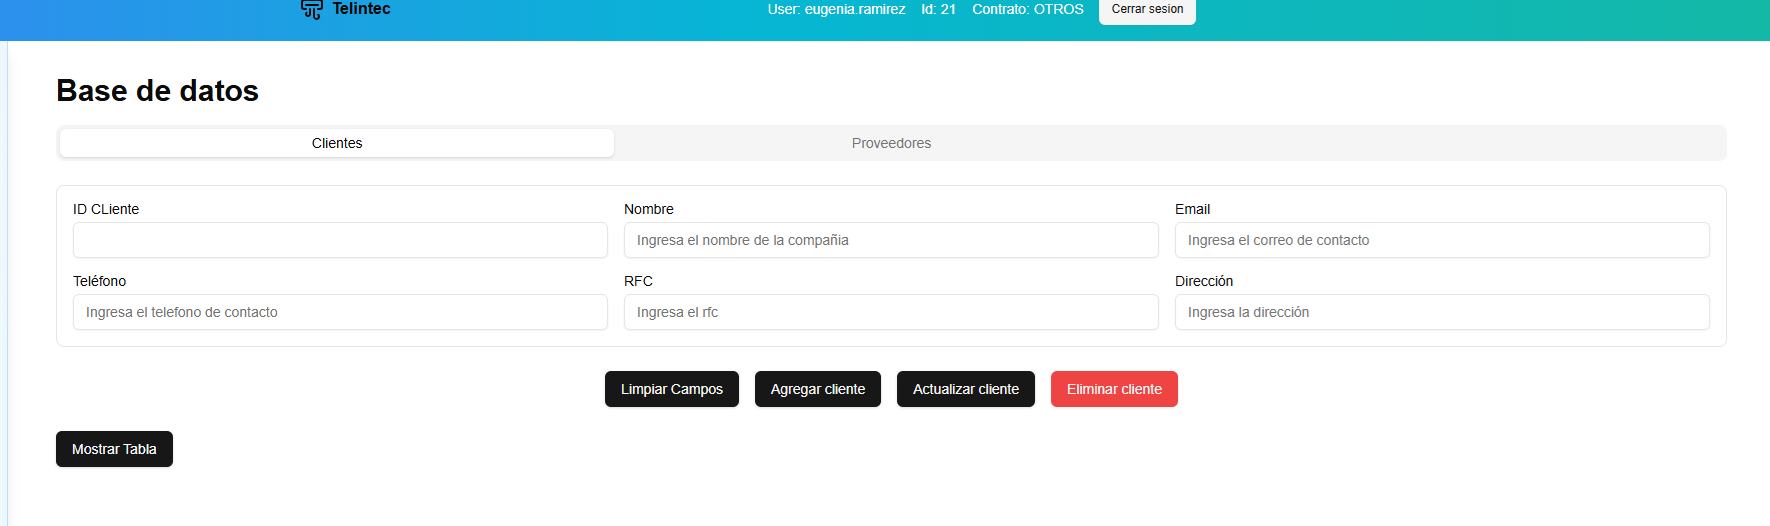
\includegraphics[width=\textwidth]{imgs/Administracion/BASE DE DATOS/administracion-BASEDEDATOS/ad_bd_provedores_tabla.png}
    \caption{Gestión de clientes.}
    \label{fig:admin1}
\end{subfigure}
\caption{Interfaz de clientes en la base de datos.}
\end{figure}

\subsubsection{3.1.2 Gestión de Base de Datos – Pestaña: Proveedores}

Funciones disponibles:

\begin{itemize}
    \item Alta de proveedores.
    \item Edición de datos como razón social, RFC, contacto.
    \item Filtro por tipo de proveedor.
\end{itemize}

\begin{figure}[h]
\centering
\begin{subfigure}{0.4\textwidth}
    
\includegraphics[width=\textwidth]{imgs/no-image.png}
    \caption{Gestión de proveedores.}
    \label{fig:admin2}
\end{subfigure}
\caption{Interfaz de proveedores en la base de datos.}
\end{figure}

\subsection{3.2 Contratos}

\subsubsection{3.2.1 Crear Contrato}

Para registrar un nuevo contrato:

\begin{itemize}
    \item Ingresa nombre del cliente, número de contrato, fecha de inicio y fin.
    \item Asocia el contrato a un proyecto si aplica.
    \item Guarda el contrato para que esté disponible en otras secciones del sistema.
\end{itemize}

\begin{figure}[h]
\centering
\begin{subfigure}{0.4\textwidth}
    
\includegraphics[width=\textwidth]{imgs/no-image.png}
    \caption{Formulario de contrato.}
    \label{fig:admin3}
\end{subfigure}
\caption{Creación de contrato en el sistema.}
\end{figure}

\subsubsection{Editar contrato}

Para modificar un contrato existente:

\begin{itemize}
    \item Usa el buscador para localizar el contrato.
    \item Haz clic en “Editar”.
    \item Actualiza los campos necesarios y guarda los cambios.
\end{itemize}

\subsection{3.3 Órdenes de compra}

\subsubsection{3.3.1 Crear orden de compra desde solicitud de material (SM)}

Desde una SM aprobada:

\begin{itemize}
    \item Selecciona los productos requeridos.
    \item El sistema autocompleta los datos del proveedor y contrato.
    \item Genera la orden de compra con folio único.
\end{itemize}

\begin{figure}[h]
\centering
\begin{subfigure}{0.4\textwidth}
    
\includegraphics[width=\textwidth]{imgs/no-image.png}
    \caption{Orden desde SM.}
    \label{fig:admin4}
\end{subfigure}
\caption{Creación de orden de compra desde solicitud de material.}
\end{figure}

\subsubsection{Crear Nueva orden de compra (manual)}

También puedes crear órdenes manualmente:

\begin{itemize}
    \item Ingresa proveedor, productos, cantidades y precios.
    \item Asocia la orden a un contrato si aplica.
    \item Guarda y descarga en PDF o Excel.
\end{itemize}

\subsection{3.4 Entregas de Solicitudes de material (SM)}

\subsubsection{3.4.1 Paso 1: Seleccionar una solicitud de material (SM)}

Para entregar materiales:

\begin{itemize}
    \item Selecciona una SM pendiente.
    \item Verifica productos disponibles y faltantes.
    \item Despacha los productos desde el almacén.
\end{itemize}

\begin{figure}[h]
\centering
\begin{subfigure}{0.4\textwidth}
    
\includegraphics[width=\textwidth]{imgs/no-image.png}
    \caption{Entrega de SM.}
    \label{fig:admin5}
\end{subfigure}
\caption{Interfaz de entrega de solicitudes de material.}
\end{figure}
